%\chapter*{Введение}
%\addcontentsline{toc}{chapter}{Введение}

\newpage
\begin{center}
\textbf{\large ГЛАВА 2 \\ Модель плавления перегретых кристаллов}
\end{center}
\refstepcounter{chapter}
\addcontentsline{toc}{chapter}{ГЛАВА 2. Модель плавления перегретых кристаллов}


%\chapter{Модель плавления перегретых кристаллов}\label{ch:ch1}
\section{Плавление в системах твердых сфер: новая модель с экспериментально измеримым параметром порядка}
\label{ch2_sec3}
%Плавление - один из наиболее изученных фазовых переходов, важных для атомных, молекулярных, коллоидных и белковых систем.
%Однако в настоящее время не существует микроскопических экспериментально доступных критериев, которые можно было бы использовать для надежного отслеживания эволюции системы при переходе, дающих возможность  понять физику зародышеобразования при плавлении и эволюции фронта плавления.
%Чтобы решить эту проблему, разработана теоретическую модель в рамках теории среднего поля с использованием нового локального параметра порядка (экспериментально измеримого) -- нормированного среднеквадратичного смещения между частицами в соседних ячейках Вороного.
%Предложенная модель протестировали в ряде экспериментов с коллоидными системами и при помощи компьютерного моделирования, при различных режимах динамики частиц (броуновским и ньютоновским), и в результате и обнаружено, что она обеспечивает превосходное описание эволюции системы при пересечении линии плавления.
%Этот новый подход предоставляет широкие возможности для применения в различных областях науки, от материалов до биологии и не только.
%Следовательно, результаты этой работы обеспечивают новое руководство для теории зародышеобразования плавления и представляют широкий интерес в конденсированных средах, химической физике, физической химии, материаловедении и мягкой материи.

%\subsection{Введение}

% \begin{comment}
% Явление плавления широко распространено в природе и может быть обнаружено начиная, от атомных и молекулярных до белковых и коллоидных систем, и выходит далеко за рамки материаловедения, поэтому формулировке критериев плавления в микроскопическом масштабе уделяется значительное внимание уже не менее 100 лет.
% Один из наиболее широко используемых микроскопических подходов принадлежит Линдеману \cite{lindemann1910} и, в частности, его переосмысление Гилварри \cite{10.1103/physrev.102.308}: то, что сейчас известно как критерий Линдемана, утверждает, что плавление происходит, когда среднеквадратичное смещение атомов от их положения достигает определенной доли (обычно 0,1-0,15) межатомного расстояния.
% Популярность критерия обусловлена его простотой и интуитивно понятной способом применения, но есть и существенные недостатки, включая низкую точность в прогнозировании температуры плавления и отсутствие явного учета жидкого состояния \cite{10.1098/rspa.1991.0068}.
% Впоследствии, был введен ряд критериев, которые можно проследить до работы Гилварри \cite{10.1063/1.1426419}, в частности, с развитием современных экспериментальных и вычислительных методов, которые обеспечивают доступ к смещениям атомов.
% Однако детали структурных изменений, особенно в отношении этих критериев, остаются неуловимыми, а ряд ключевых явлений, включая детали механизма зародышеобразования, кинетики фронта плавления и поведения системы вблизи точки плавления, остаются малоизученными.
%
% В то же время эксперименты с разрешением отдельных частиц с модельными системами, сопровождаемыми молекулярно-динамическим (МД) моделированием, позволяют с предельной детализацией наблюдать фазовые переходы в различных режимах, от слабых до сильно неравновесных. \cite{book.ivlev}.
% Исследования коллоидов с разрешением отдельных частиц позволили изучить широкий круг явлений \cite{10.1038/natrevmats.2015.11, 10.1039/c9sm01953g}, включая плавление и кристаллизацию \cite{10.1126/science.1112399, 10.1038/ncomms8110, 10.1038/ncomms7942, 10.1063/1.2189850, 10.1039/c5cp07943h, 10.1039/c2sm26473k, 10.1103/physrevlett.118.088003, 10.1039/c4sm02193b, 10.1039/c2sm27654b, 10.1002/smll.201802049, 10.1103/physrevlett.119.128001},
% фазовые переходы кристалл-кристалл \cite{10.1038/ncomms14978, 10.1103/physrevlett.119.128001, 10.1039/c5sm01551k},
% конденсацию и критические явления \cite{10.1038/nphys679},
% гелеобразование и стеклообразное состояние \cite{10.1016/j.physrep.2014.11.004, 10.1063/1.5000263, 10.1063/1.4794695},
% переохлажденные жидкости \cite{10.1126/science.287.5453.627}.
% В частности, был выполнен ряд исследований с использованием коллоидных сфер термочувствительного микрогеля N-изопропилакриламида (NIPAm) (диаметр которых уменьшается с повышением температуры),
% в том числе предплавление на дефектах \cite{10.1126/science.1112399},
% огрубление границ зерен \cite{10.1103/physrevx.8.021045},
% поликристаллические структуры \cite{10.1103/physrevx.8.041023},
% двухступенчатая нуклеация при фазовых переходах кристалл-кристалл \cite{10.1038/nmat4083},
% и плавление в перегретых кристаллах \cite{10.1126/science.1224763}.
% Подобно коллоидам, исследования с разрешением отдельных частиц с комплексной (пылевой) плазмой (заряженные микрочастицы в ионизированном газе \cite{10.1039/c0sm00813c}) успешно позволили исследовать плавление и кристаллизацию \cite{10.1103/physrevlett.80.5345, 10.1103/physrevlett.105.115004, 10.1038/nphys242},
% спинодальный распад \cite{10.1103/physrevlett.105.045001, 10.1103/physrevlett.116.115002},
% стекловидное состояние \cite{10.1209/0295-5075/123/35001, 10.1103/physreve.91.052301},
% эволюцию кристаллических доменов \cite{10.1103/physrevlett.124.165001},
% возбуждения в жидкостях \cite{10.1103/physrevlett.97.115001, 10.1021/acs.jpclett.9b03568},
% термическую активацию и распространение неравновесных фронтов плавления \cite{10.1103/physreve.96.043201, 10.1103/physreve.97.043206, 10.1103/physrevlett.121.075003} (тесно связанных с диссипативными фазовыми переходами между термически активированным и неактивированным состояниями \cite{10.1039/c8sm01836g, 10.1103/physreve.100.023203}).
% Таким образом, значительное понимание общих механизмов плавления кристаллов может быть получено с помощью модельных систем \cite{book.ivlev, 10.1039/c0sm00813c}.
%
% В этом контексте общая теоретическая основа, которая может связывать модельные системы, а также реальные материалы с компьютерным моделированием с разрешением отдельных частиц (например, МД), будет представлять значительный практический интерес.
% Однако некоторые вопросы, возникающие в результате исследований с разрешением отдельных частиц, остаются без ответа:
% Может ли такая модель быть основана на микроскопических параметрах, экспериментально доступных в реальных (то есть атомных и молекулярных) системах?
% Могут ли эти явления быть описаны одинаково в системах с разными динамическими режимами (например, броуновский в белках и коллоидах и ньютоновский в пылевой плазме и атомных системах)?
% Как далеко (если это вообще справедливо) физическая аналогия между неравновесными явлениями в слабодемпфированных (сложная плазма) и сильнодемпфированных (коллоиды, белки) системах распространяется на плавление в атомных системах?
% \end{comment}

Были проведены исследования, направленные на развитие методик описания плавления -- явления, широко представленного в природе и технологиях. В результате была разработана новая теоретическая модель среднего поля (представленная в настоящем разделе) для описания плавления в микроскопическом масштабе и применена для изучения распространения фронтов плавления в перегретых кристаллах во время роста зародышей.
Предложенная модель основана на новом локальном параметре порядка -- среднеквадратичном отклонении расстояний между частицами соседних ячеек Вороного, тем самым данный параметр порядка вводит локальные корреляции в модель среднего поля.
Обнаружено, что предложенный подход обеспечивает точное описание плавления перегретых коллоидных (NIPAm) систем и модельных кристаллов, смоделированных методом МД, несмотря на значительные различия в динамике (броуновская и ньютоновская).
Установлено, что предложенная модель проявляет богатый спектр динамических режимов, включая бифуркационное поведение (в процессе гомогенного зародышеобразования) на начальных стадиях плавления, а также демонстрирует аналогию с моделью \cite{10.1103/physreve.96.043201, 10.1103/physreve.100.023203}, описывающей тепловую эволюцию в химически реактивных средах и в комплексных (пылевых) плазменных кристаллах.
Это позволяет предполагать, что предложенная модель будет обладать широким спектром применения, от атомных и молекулярных кристаллов до коллоидных и белковых систем.

%\subsection{материалы и методы}

%\subsubsection{$\lambda^2$-Параметр: Локальная мера беспорядка}
%\label{SSMF-AppA}

В работе~\cite{10.1021/acs.jpcc.7b09317}, для характеризации локальной разупорядоченности и идентификации конденсированных (жидких или твердых) фаз в конденсируемых системах был предложен подход, основанный на анализе ячеек Вороного -- элементарной площади (``объема''), занимаемой каждой частицей в системе.
В рамках подхода на первом этапе система разбивается на ячейки Вороного, чтобы вычислить следующий параметр:
\begin{equation}
\label{SSMF-eq1}
\sigma_{i} =\frac{1}{a_i N_{ni}}\sqrt{\sum_{j<k}^{N_{ni}}{(r_{ij}-r_{ik})^2}/2}, \quad r_{ij}=|\mathbf{r}_i-\mathbf{r}_j|,
\end{equation}
где $\mathbf{r}_i$ -- радиус-вектор $i$-ой частицы, $N_{ni}$ -- количество соседних ячеек, $a_i = \sqrt{S_i/\pi}$ -- характерный радиус, $S_i$ -- площадь ячейки Вороного.
На втором этапе для подавления сильных локальных тепловых флуктуаций проводится усреднение с соседними ячейками, которые имеют общую грань (сторона в 2D случае) с ячейкой частицы $i$ \cite{10.1021/acs.jpcc.7b09317}:
\begin{equation}
\label{SSMF-eq2}
\lambda_{i} = \frac{1}{N_{ni}+1}\left(\sigma_{i}+\sum_{j=1}^{N_{ni}}{\sigma_{j}}\right).
\end{equation}
В результате получается стандартное отклонение $\lambda_i^2$ расстояний между соседними частицами в \emph{физически малом объеме} в окрестности $i$-й частицы.
Важно отметить, что $\lambda_i^2$ одинаково хорошо применимо для характеризации как твердой, так и жидкой фаз системы, поскольку этот параметр связан с локальным беспорядком в физически малом объеме \cite{10.1021/acs.jpcc.7b09317}.
\textcolor{red}{В кристаллах $\lambda^2$ связано с параметром Линдемана для соседних частиц \cite{10.1016/0375-9601(85)90617-6}, поскольку $\lambda^2 \propto \sigma_\|^2$, где $\sigma_\|^2$ - продольная компонента среднеквадратичного смещения ближайших частиц.
Кроме того, $\sigma_\|^2$ играет важную роль в вычислении первого корреляционного пика в кристаллах \cite{10.1063/1.4869863, 10.1063/1.4926945, 10.1088/0953-8984/28/23/235401, 10.1039/c7sm02429k, 10.1063/1.5116176}.}

%\subsubsection{Детали эксперимента NIPAm}
%\label{SSMF-AppB}

Для изучения плавления в перегретых кристаллах были выполнены эксперименты аналогично тому, как это было сделано в работе~\cite{10.1126/science.1224763}.
Для создания трехмерных стабильных коллоидных кристаллов использовались суспензии термочувствительных коллоидных сфер NIPAm в водном растворе с 1 $mM$ уксусной кислоты.
К образцу было добавлено небольшое количество нефлуоресцентного красного красителя, 0,2\% по объему, для поглощения тепла.
Эффективный диаметр частиц изменяется линейно от
$1.04 \; \mathrm{\mu m} $ при $ 25 ^ {\circ} \mathrm{C}$ до $0.89 \; \mathrm{\mu m}$ при $30 ^ {\circ}\; \mathrm{C}$ в воде.

Коллоидный образец размещался в стеклянном капиллярном канале размером $\sim 18 \times 3 \times 0.1 \; \mathrm{mm ^ 3} $ и выдерживался в состоянии покоя достаточно долго, чтобы сформировать поликристалл только с малым числом доменов.
Показатели преломления частиц и растворителя совпадали, что позволило визуализировать кристаллический слой в середине системы с помощью светлопольной микроскопии.
При повышении температуры, из-за лазерного нагрева системы, объемная доля, занимаемая частицами, уменьшалась, вызывая плавление образца \cite{10.1126/science.1112399}.
Более подробная информация об экспериментах представлена в работе~\cite{10.1126/science.1224763}.

%\subsubsection{Детали моделирования МД}
%\label{SSMF-AppC}

Для дополнения экспериментов с коллоидами, в которых частицы движутся в броуновском (сверхзатухающем) режиме, проведено МД-моделирование кристаллов в условиях ланжевеновской динамики.
В качестве характерного примера рассмотрена система частиц, взаимодействующих по обратному степенному закону (IPL18):
\begin{equation}
\label{SSMF-eq3}
\varphi(r) = \epsilon a \left(\frac{\sigma}{r}\right)^{18},
\end{equation}
где $\epsilon$ и $\sigma$ -- сила и характерный масштаб отталкивания соответственно,
а параметр $ a = 2.365 $ введен для удобства моделирования скачкообразного изменения диаметра частиц.
Использовалась нормированная температура $ T/ \epsilon \rightarrow T $, расстояние $ r/ \sigma \rightarrow r $, плотность частиц $\rho\sigma^3/m\rightarrow n$ и время $t\sqrt{\epsilon/m\sigma^2} \rightarrow t$ ($m$ -- масса частицы).

Для анализа плавления перегретого кристалла выполнено МД-моделирование системы, состоящей из $ N = 7.2 \times 10 ^ 4 $ частиц в $NVT$ ансамбле при $n=0.867$ и $T=1$.
В исходном состоянии частицы располагались в ГЦК решетке, ориентированной таким образом, чтобы плоскость (111) совпадала с горизонталью.
Размеры области моделирования в $ x $, $ y $ и $ z $ -направлениях были выбраны так, чтобы $ L_x / L_z \approx 20.4 $ и $ L_y / L_z \approx 21.3 $.
Временной шаг был выбран равным $ \Delta t = 7.4 \times 10 ^ {- 4} \sqrt {m \sigma ^ 2 / \epsilon} $. Расчеты методом молекулярной динамики проводились в открытом программном пакете LAMMPS.
Моделирование проводилось в 2 этапа: (i) система моделировалась на протяжении $ 10 ^ 5 $ временных шагов с $ a = 7.224 $ для достижения состояния равновесия; (ii) значение $a$ фиксировалось равным $ 2.365 $ и проводилось дополнительное моделирование на $ 4 \times 10 ^ 5 $ шагов для анализа плавления в кристалле.

%\subsection{Результаты}
%\subsubsection{Самосогласованная модель среднего поля эволюции $\lambda^2$ - поля}

Примеры кристаллических и жидких структур показаны на Рис.~\ref{SSMF-Figure1}(a) и \ref{SSMF-Figure1}(b) соответственно.
Белые точки -- это частицы, ячейки Вороного показаны сплошными серыми линиями, и окрашены в соответствии со значением параметра $\lambda^2$ -- нормированным среднеквадратичным смещением между частицами в соседних ячейках Вороного \cite{10.1021/acs.jpcc.7b09317}. %(см. раздел~\ref{SSMF-AppA}).
В кристаллах $\lambda^2$ связано с параметром Линдемана для соседних частиц \cite{10.1016/0375-9601(85)90617-6}.
Это обусловлено тем, что $\lambda^2\propto \sigma_ \| ^ 2 $, где $ \sigma_ \| ^ 2 $ является продольной составляющей среднеквадратичного смещения ближайших частиц.
Кроме того, $ \sigma_ \| ^ 2 $ играет важную роль в вычислении первого корреляционного пика в кристаллах \cite{10.1063/1.4869863, 10.1063/1.4926945, 10.1088/0953-8984/28/23/235401, 10.1039/c7sm02429k, 10.1063/1.5116176}.
После плавления кристаллическая решетка разрушается, но, несмотря на диффузию частиц, разбиение Вороного все еще применимо в жидкости.

В случае систем с отталкиванием, рост $\lambda^2$ обеспечивается (i) повышением температуры или (ii) уменьшением плотности.
В то время как первый механизм играет центральную роль в системах с мягким отталкиванием между частицами (например, в мягких кристаллах при низких температурах $\lambda^2\propto T $), последний является определяющим в системах типа твердых сфер (таких как коллоиды NIPAm), коллективная динамика которых определяется объемной долей частиц.
В обоих случаях $\lambda^2$ играет роль параметра порядка, и в этих терминах плавление представляет собой переход от состояний с малым $\lambda^2$ (кристалл) к состояниям с большим $\lambda^2$ (жидкость).

Чтобы получить самосогласованную модель эволюции $ \lambda^2$-поля,
необходимо рассмотреть слабо неоднородное пространственное поле $\lambda^2$.
Параметр $\lambda ^ 2$ неконсервативен, а следовательно его эволюция определяется нестационарным уравнением Гинзбурга-Ландау (или моделью Ланжевена) \cite{book.desai}:
\begin{equation}
\label{SSMF-eq4}
\frac{\partial \lambda^2}{\partial t} = -\Gamma \frac{\delta \mathcal{F}}{\delta \lambda^2} + \varepsilon^{1/2}\xi(t,\mathbf{r}),
\end{equation}
где $\Gamma$ -- обобщенная вязкость, $ \mathcal{F} $ -- функционал свободной энергии системы, $\langle \xi(t,\mathbf{r})\xi(t',\mathbf{r}')\rangle = \delta(t-t')\delta(\mathbf{r}-\mathbf{r}')$ и $\varepsilon = 2k_BT\Gamma$.
Последнее слагаемое в~\eqref{SSMF-eq2} описывает тепловые флуктуации поля $\lambda^2$.

\begin{figure}[!t]
\centering
 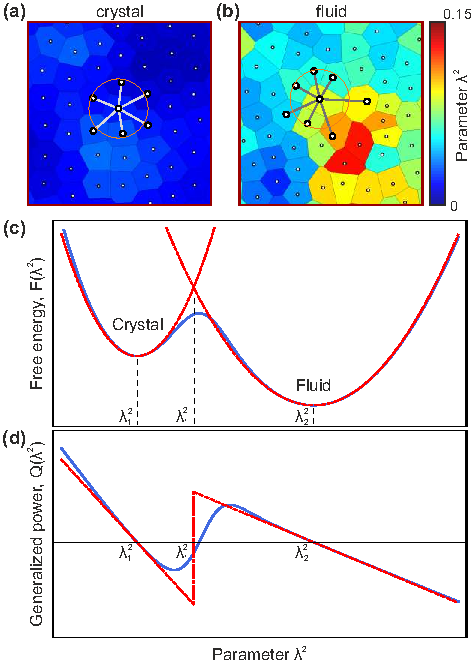
\includegraphics[width=100mm]{SSMF-Figure1.pdf}
 \caption{\textbf{Схематичное изображение к предлагаемой самосогласованной $\lambda^2$~-~модели:}
 (a) и (b) снимки системы в кристаллическом и жидком состоянии (взяты из МД моделирования).
  Ячейки Вороного раскрашены в соответствии со значениями параметра $ \lambda^2$.
  Панели (c) и (d) схематично иллюстрируют (синие линии) зависимость свободной энергии $ F (\lambda ^ 2) $ (в однородной системе) и обобщенную мощность $ Q (\lambda ^ 2) $, сопряженную с полем $\lambda^2$.
 Пунктирные красные линии иллюстрируют ступенчатое приближение \eqref{SSMF-eq5} и \eqref{SSMF-eq7}.
 }
\label{SSMF-Figure1}
\end{figure}

\begin{figure*}[!t]
\centering
 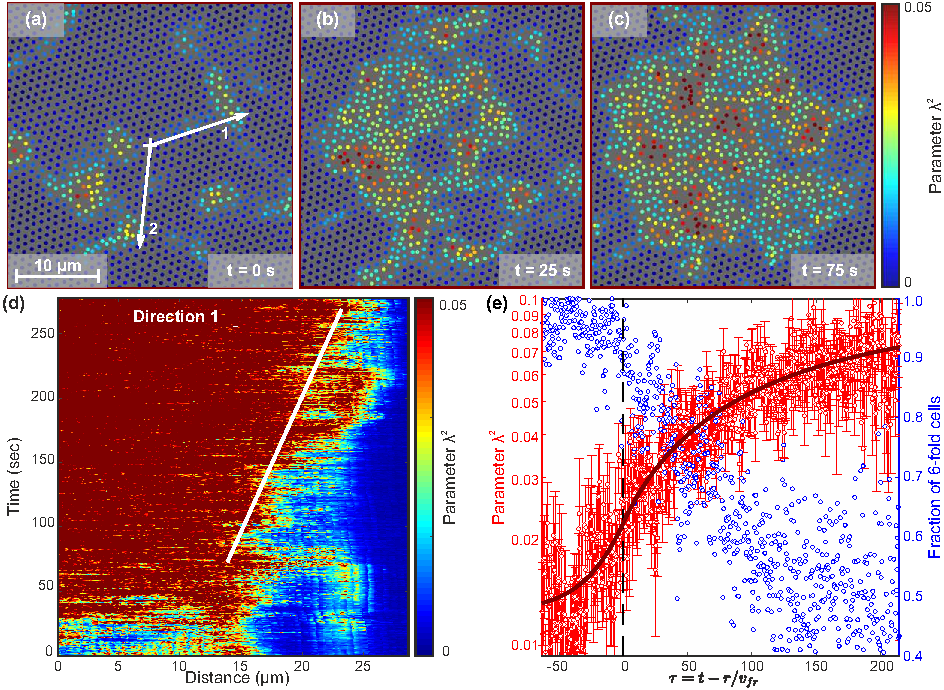
\includegraphics[width=160mm]{SSMF-Figure2.pdf}
 \caption{\textbf{Экспериментальное наблюдение автомодельного $\lambda^2$-профиля распространяющегося фронта плавления в коллоидном кристалле при промежуточной степени перегрева:}
 (a) - (c) Последовательные снимки системы, где круги представляют собой частицы, окрашенные в соответствии со значением $\lambda^2$.
 (d) Эволюция поля $\lambda^2(r, t)$ в радиальном направлении (1), показанном на (a).
 (e) $\lambda^2(\tau)$ -- профиль распространяющегося фронта плавления при росте зародышей.
 Красные символы -- экспериментальные точки, красная сплошная линия -- теоретическая аппроксимация \eqref{SSMF-eq9}.
 Синие символы представляют собой долю ячеек Вороного с 6-ю соседями в плоскости анализа, а резкое падением, указывает на разрушение кристаллической структуры.}
\label{SSMF-Figure2}
\end{figure*}

\begin{figure*}[!t]
\centering
 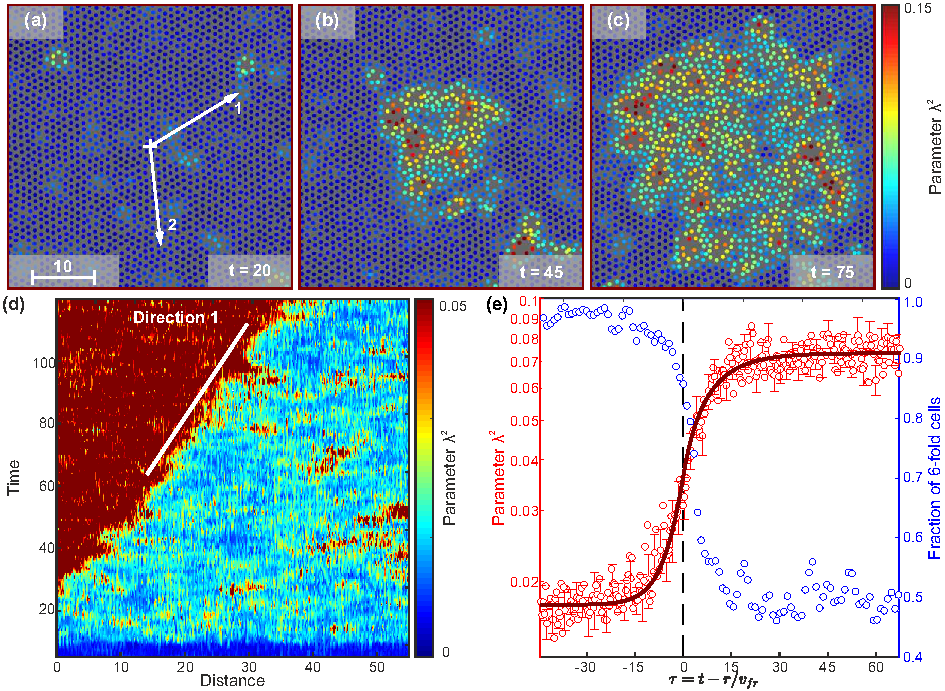
\includegraphics[width=160mm]{SSMF-Figure3.pdf}
 \caption{\textbf{Автомодельный $ \lambda^2$-профиль распространяющегося фронта плавления в перегретом кристалле, наблюдаемый при МД-моделировании:} Описание такое же, как на Рис.~\ref{SSMF-Figure2}.}
\label{SSMF-Figure3}
\end{figure*}

Функционал свободной энергии $\mathcal{F}[\lambda^2] = \int{d\mathbf{r}\;F[\lambda^2]}$ в квадратичном приближении может быть представлен в виде:
\begin{equation}
\label{SSMF-eq5}
F[\lambda^2] = F_{\mathrm{1,2}}^{(0)}+\frac{1}{2}A_{1,2}\left(\lambda^2-\lambda_{1,2}^2\right)^2 + \frac{1}{2}\alpha_{1,2}\left(\nabla\lambda^2\right)^2,
\end{equation}
где $F_{1,2}^{(0)}$ -- энергия однородного состояния ($1$ или $2$), $A$ и $\alpha$ -- положительные коэффициенты разложения \cite{book.desai}, а индексы $ 1 $ и $ 2 $ соответствуют кристаллическому или жидкому состоянию при $\lambda^2 \lessgtr \lambda_\ast^2$ соответственно.
Параметр $\lambda_\ast^2 $ -- это порог, связанный с обобщенным критерием плавления типа Линдемана, и предполагается, что $ F_{\mathrm{1}} ^ {(0)}> F_{\mathrm{2}} ^ {(0)} $ для рассматриваемого случая.

При помощи уравнений~\eqref{SSMF-eq4} и \eqref{SSMF-eq5} можно получить:
\begin{equation}
\label{SSMF-eq6}
\frac{\partial \lambda^2}{\partial t} = \chi_{1,2} \nabla^2\lambda^2 + Q(\lambda^2) +  \varepsilon^{1/2}\xi(t,\mathbf{r}),
\end{equation}
где $ \chi_{1,2} = \alpha_{1,2} \Gamma $ -- характеризует диффузию $\lambda^2$,
а $ Q (\lambda ^ 2) $ -- обобщенный источник $ \lambda^2$-поля,
\begin{equation}
\label{SSMF-eq7}
Q(\lambda^2) =
\left\{
  \begin{array}{ll}
   -\gamma_{1}\left(\lambda^2-\lambda_{1}^2\right), & \lambda^2  < \lambda_\ast^2;\\
   -\gamma_{2}\left(\lambda^2-\lambda_{2}^2\right), & \lambda^2 > \lambda_\ast^2,\\
  \end{array}
\right.
\end{equation}
где $\gamma_{1,2} = \Gamma A_{1,2}$.
Уравнение \eqref{SSMF-eq6} демонстрирует аналогию с эволюцией температуры в химически реактивных средах \cite{10.1088/0004-637x/805/1/59} и совпадает с уравнением для кинетической температуры, которое исследовалось в работах~\cite{10.1103/physreve.96.043201, 10.1103/physreve.97.043206, 10.1103/physreve.100.023203} при анализе распространяющихся фронтов неравновесного плавления в однослойных пылевых плазменных кристаллах.

Энергия \eqref{SSMF-eq5} для однородного случая и соответствующая обобщенная мощность $ Q (\lambda ^ 2) $ показаны на Рис.~\ref{SSMF-Figure1}(с) и \ref{SSMF-Figure1}(d).
Как видно на Рис.~\ref{SSMF-Figure1}(d), система может существовать долгое время в окрестности устойчивых состояний с $\lambda^2= \lambda_{1,2} ^ 2 $, тогда как пороговое значение $\lambda^2=\lambda_\ast^2$ соответствует неустойчивой точке.
Ниже будет показано, что решение уравнения~\eqref{SSMF-eq6} объясняет два важных явления, изучаемых в настоящем исследовании:
(i) распространение автомодельных фронтов плавления в перегретых кристаллах, образованных частицами, движущимися в броуновском или ньютоновском динамическом режиме, и (ii) бифуркационное поведение различных $\lambda^2$ -флуктуаций (зародышей плавления) в перегретом кристалле.

Если пренебречь влиянием теплового шума и полагать кривизну фронта плавления незначительной при его распространении, то это означает, что $ \epsilon \simeq 0 $ и в уравнении~\eqref{SSMF-eq6} можно записать $ \nabla ^ 2 = \partial ^ 2 / \partial r ^ 2 $.
В этом случае, самоподобный профиль (бегущей волны плавления) описывается функцией $\lambda^2(t-r/v_\mathrm{fr})\equiv \lambda^2(\tau)$ (где $v_\mathrm{fr}$ -- скорость фронта), которая подчиняется уравнению:
\begin{equation}
\label{SSMF-eq8}
\frac{\chi_{1,2}}{v_{\mathrm{fr}}^2} \frac{d^2 \lambda^2}{d\tau^2} -\frac{d \lambda^2}{d \tau} -\gamma_{1,2}(\lambda^2-\lambda_{1,2}^2) =0,
\end{equation}
учитывая, что $\lambda^2(\tau) $ и его производная $ d\lambda^2/ d \tau $ должны быть непрерывными в точке $ \tau = 0 $, где $\lambda^2=\lambda_\ast^2$.
Полученное уравнение идентично уравнению, которое возникает в задаче неравновесного плавления в комплексных (пылевых) плазменных кристаллах, а следовательно, решение уравнения~\eqref{SSMF-eq8} аналогично \cite{10.1103/physreve.96.043201, 10.1103/physreve.100.023203}:
\begin{equation}
\label{SSMF-eq9}
\frac{\lambda^2(\tau)-\lambda^2_1}{\lambda^2_\ast-\lambda^2_1}=
\left\{
  \begin{array}{ll}
    e^{p_1 \tau}, & \tau < 0;\\
   1+\left(1-e^{-p_2\tau}\right)p_1/p_2 , & \tau > 0,\\
  \end{array}
\right. \\
\end{equation}
где $ p_{1,2} = \left(\sqrt {1 + 4 \gamma_{1,2} \chi_{1,2} / v_\mathrm{fr} ^ 2} \pm 1 \right) v_\mathrm{fr} ^ 2/2 \chi_{1,2} $ -- показатели в экспоненциальных ветвях решения до и после фронта плавления.
В пределе $\tau \gg 1$, $\lambda^2(\tau) \rightarrow \lambda_2^2$, откуда следует, что
$\left(\lambda_2^2-\lambda^2_1\right)/\left(\lambda^2_\ast-\lambda^2_1\right) = (1+p_1/p_2)$.
Скорость фронта плавления и показатели $p_{1,2} $ (неизвестные \emph{априори}) сложным образом определяются диффузией $\lambda^2$, спецификой межчастичных взаимодействий и различием химических потенциалов на границе жидкость-твердое тело~\cite{10.1038/ncomms7942}.
%Далее по тексту, будет показана эффективность описания эволюции $\lambda^2$-поля в рамках  предложенной модели на примере коллоидного кристалла NIPAm и МД моделирования, чтобы доказать, что она адекватно описывает эволюцию поля $\lambda^2$ и распространение фронтов плавления в перегретых кристаллах.

%\subsubsection{Прямое наблюдение автомодельного профиля устойчивых фронтов плавления в перегретых коллоидах}
%\label{SSMF-Results-Experiment}

Первый вывод, следующий из уравнения~\eqref{SSMF-eq6} (с $ \varepsilon = 0 $), заключается в том, что самоподобный профиль $\lambda^2(\tau) $ представляет собой комбинацию двух \emph{экспоненциальных ветвей} \eqref{SSMF-eq9}.
Это утверждение может быть подтверждено на основе экспериментов с коллоидами NIPAm частиц.
Эта коллоидная система ведет себя как модельная система твердых сфер \cite{10.1126/science.1224763, 10.1038/ncomms7942}.
Модель твердых сфер представляет собой простейшее взаимодействие между двумя частицами с единственным ограничением: две частицы не могут проникать друг в друга.
Все возможные конфигурации имеют нулевую потенциальную энергию, что означает, что свободная энергия полностью определяется энтропией.
Следовательно, единственным параметром, определяющим фазовое состояние (и другие свойства системы), является объемная доля частицы $ \phi = N V_p / V $, представляющая безразмерный аналог численной плотности частиц (где $ N $ -- количество частиц, $ V_p $ -- объем отдельной частицы, а $ V $ -- полный объем системы).
В то же время объемную долю можно регулировать с помощью лазерного нагрева коллоидной системы NIPAm в эксперименте, путем изменения объема частиц при нагреве.

Результаты эволюции поля $\lambda^2$ и автомодельных фронтов плавления в кристалле NIPAm показаны на Рис.~\ref{SSMF-Figure2}.
Для изучения распространяющихся фронтов плавления коллоидный ГЦК кристалл NIPAm частиц был нагрет при помощи лазерного излучения и был визуализирован слой, нормальный к направлению [111].
В этой плоскости частицы в ГЦК-кристалле формируют гексагональный кристалл, который разрушается во время плавления, как показано на Рис.~\ref{SSMF-Figure2}(a)-\ref{SSMF-Figure2}(c), где частицы окрашены в соответствии со значениями $ \lambda^2$.
В отличие от параметра Линдемана, $\lambda^2$ имеет конечное значение как в кристалле, так и в жидкости, и нечувствителен к выходу частиц из области наблюдения.

Эволюцию параметра $\lambda^2$ была проанализирована на разных расстояниях вдоль направления (1) на Рис.~\ref{SSMF-Figure2}(a), таким же образом, как описано в работах~\cite{10.1103/physreve.96.043201, 10.1103/physreve.100.023203}.
Эволюция $\lambda^2$ в направлении 1 показана на Рис.~\ref{SSMF-Figure2}(d).
На представленных графиках видно образование зародыша жидкости с радиусом $\simeq 15\;\mathrm{\mu m}$ и его последующий рост, что отображается в виде перехода от синей к красной области в $\lambda^2$.
Сплошная белая линия соответствует скорости фронта плавления $v_{\mathrm{fr}}\simeq 0.05 \;\mathrm{\mu m /s}$.

Наблюдаемый режим плавления был описан в работе~\cite{10.1038/ncomms7942} как \emph{промежуточный перегрев}.
В этом режиме рост жидкого зародыша аналогичен таковому при слабом перегреве (фронт плавления распространяется последовательно, с редкими "скачками", вызванными зарождением новых зародышей перед фронтом), но несмотря на это, скорость фронта зависит от величины характеризующей степень ``перегрева''  $\Delta \phi = \phi_m - \phi $  нелинейно, где $ \phi_m = 54,5 \% $ -- объемная доля соответствующая плавлению.
Чтобы обосновать это, были использованы частицы с диаметром в$ \sim 1.33$  раза  больше, чем в работе~\cite{10.1038/ncomms7942} ($ 1.04 \; \mathrm{\mu m} $ против $ 0.78 \; \mathrm{\mu m} $ при $ 25 ^ {\circ} \mathrm{C} $), тогда как $ v_{\mathrm{fr}} $ пропорционален размеру частиц.
Учитывая соответствие экспериментов с частицами разного размера, в рассмотренном случае получается $ \Delta \phi = \phi_m - \phi \simeq 3.5 \% $ (это соответствует $ v_{\mathrm{fr}} \simeq 0.05 /1.33 = 0,037 \; \mathrm{\mu m / s} $ для более мелких частиц, см. Рис. 3c в работе~\cite{10.1038/ncomms7942}).
Кроме того, эволюция поля $\lambda^2$ на Рис.~\ref{SSMF-Figure2} наглядно демонстрирует набор особенностей, присущих промежуточному перегреву, включая спонтанное образование и исчезновение малых (нежизнеспособных) зародышей, а также сильных колебаний фронта на Рис.~\ref{SSMF-Figure2} (d), вызванных тепловыми флуктуациями, вклад которых становится существенным для системы в окрестности фазового перехода, в соответствии с результатами, приведенными в работах~\cite{10.1039/c7sm02291c, 10.1063/1.5059358}.

Для получения параметров автомодельного $ \lambda^2$-профиля, необходимых для последующего сравнения с рассматриваемой моделью, были усреднены временные зависимости $\lambda^2(\tau) \equiv \lambda^2(t-r/v_{\mathrm{fr}})$, рассчитанные на разных расстояниях от центра, показанного крестом на Рис.~\ref{SSMF-Figure2}(a) (10 точек, равномерно распределенных по линии 1, от $20$ до $30\; \mathrm{\mu m}$).
Экспериментально полученный профиль для $\lambda^2(\tau) $ показан на Рис.~\ref{SSMF-Figure2} (e) красными точками.
Синие символы обозначают количество ячеек с 6 гранями в плоскости анализа.
Сплошная красная линия -- самоподобный профиль, полученный с использованием уравнения~\eqref{SSMF-eq9}, параметры которого ($p_{1,2}$ и $ \lambda_\ast ^ 2$) были найдены методом наименьших квадратов, при минимизации расхождений между экспериментальными и теоретическим точками ($ \lambda_1 ^ 2 $ рассчитано при анализе кристалла перед плавлением).
Таким образом были определены значения $\lambda^2$, соответствующие кристаллическому, жидкому и пороговому состояниям: $ \lambda_1 ^ 2 \simeq 0.015 $, $ \lambda_2 ^ 2 \simeq 0.07 $ и $\lambda_\ast^2\simeq 0,025 $ соответственно.

Теоретический автомодельный профиль (красная линия на Рис.~\ref{SSMF-Figure2} (e)) хорошо согласуется с экспериментальными данными, что подтверждает предложенную самосогласованную $\lambda^2$-модель.
Точка перехода (вертикальная пунктирная линия на Рис.~\ref{SSMF-Figure2} (e)) между экспоненциальными ветвями профиля $ \lambda^2$ показывает точную корреляцию с началом интенсивного спада в доле 6-угольных ячеек Вороного в плоскости анализа, это указывает на то, что структура разрушается и эволюционирует от низкого к высокому $\lambda^2$-состоянию, как было объяснено на примере Рис.~\ref{SSMF-Figure1}.

%\subsubsection{Прямое наблюдение автомодельного профиля стационарных фронтов плавления в МД симуляции}
%\label{SSMF-Results-MD}

Распространение фронтов плавления -- медленный процесс по сравнению с характерным временем движения отдельных частиц.
Это означает, что описание в терминах медленно флуктуирующего $\lambda^2$-поля должно быть применимым как в коллоидах, демонстрирующих броуновский режим движения отдельных частиц, так и в системах с ланжевеновской динамикой.
Чтобы подтвердить, что все ключевые особенности, наблюдаемые в случае коллоидных систем, присутствуют и в атомарных кристаллах было выполнено моделирование аналогичного процесса методом МД с термостатом Ланжевена и слабым затуханием.
При параметрах выполненного МД-моделирования плотность системы при плавлении и кристаллизации (в безразмерных единицах) составляет $ n_m = 0,93 $ и $ n_f = 0,88 $, соответственно~\cite{10.1080/00268979500100911}.
Следовательно, ступенчатое изменение диаметра частиц в проведенных расчетах можно оценить как $ (n_f / n) ^ {1/3} -1 \simeq 0.5 \% $ ($ n = 0.867 $), это позволяет вычислить падение эффективной объемной доли частиц относительно ее значения, соответствующего плавлению, как
$\Delta \phi  \simeq (n_m/n)^{1/3}-1\simeq 2.4\%$.
Полученное значение близко к режиму промежуточного перегрева, обсуждаемому в работе~\cite{10.1038/ncomms7942}.
%Прямое соответствие режимов перегрева в твердых сферических коллоидах и системах частиц, взаимодействующих с более мягкими потенциалами, выходит за рамки настоящей работы и требует изучения в будущем.

Результаты проведенного МД-моделирования автомодельных фронтов плавления в перегретом кристалле частиц с IPL18 взаимодействием представлены на Рис.~\ref{SSMF-Figure3}.
Параметры профиля $\lambda^2$ на Рис.~\ref{SSMF-Figure3} (e) немного отличаются по сравнению с Рис.~\ref{SSMF-Figure2}(e).
Полученные значения $\lambda^2$ в кристаллическом, жидком и пороговом состояниях равны $\lambda_1^2 \simeq 0.01$, $\lambda_2^2 \simeq 0.07$, и $\lambda_\ast^2 \simeq 0.035$, соответственно.
Значения $\lambda_\ast^2$, полученные в МД и в эксперименте, хорошо согласуются с критерием Линдемана для ближайших соседей \cite{10.1016/0375-9601(85)90617-6}.
В частности, $L\simeq \sqrt{\lambda_\ast ^ 2/2} $, что дает около $ 11 \% $ и $ 13 \% $ для экспериментов и моделирования, соответственно.

Таким образом, несмотря на различные динамические режимы, результаты моделирования методом МД демонстрируют высокий уровень сходства с коллоидным экспериментом.
Более того, флуктуации фронта плавления при моделировании очень похожи на экспериментальные и согласуются с предыдущими исследованиями \cite{10.1038/ncomms7942} в терминах предложенного $\lambda^2$-подхода.

\begin{figure}[!t]
\centering
 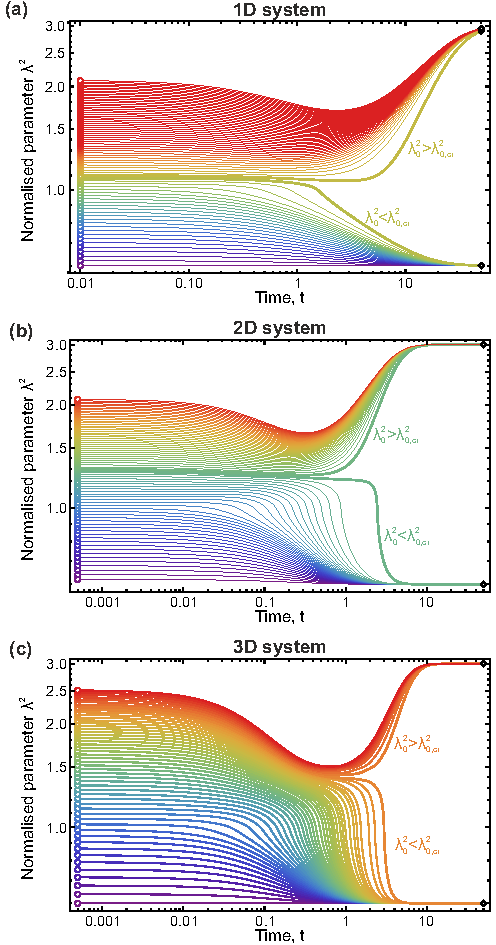
\includegraphics[width=100mm]{SSMF-Figure4.pdf}
 \caption{\textbf{Бифуркационное поведение при различных начальных флуктуациях \eqref {SSMF-eq11}, описываемое самосогласованной моделью эволюции $\lambda^2$}:
 Зависимости $\lambda^2(t, 0)$ при начальных значениях $ \lambda^2(0,0)\equiv\lambda_0 ^2\gtrless\lambda_{0,\mathrm {cr}}^2$ показаны для (a) 1D, (b) 2D \textcolor{red}{и (с) 3D систем}. Бифуркационное поведение отчетливо себя проявляет, благодаря качественному изменению вида $\lambda ^ 2(t,0)$ при малом изменении начального состояния в окрестности $\lambda_ {0,\mathrm{cr}}^2$.}
\label{SSMF-Figure4}
\end{figure}


\begin{figure*}[!t]
\centering
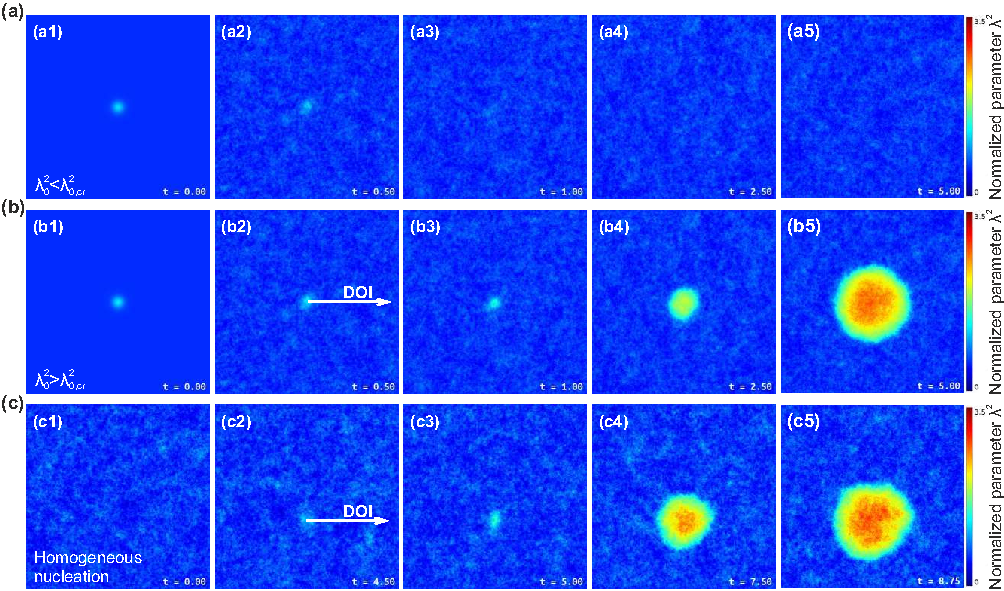
\includegraphics[width=170mm]{SSMF-Figure5.pdf}
 \caption{\textbf{Эволюция различных начальных $\lambda^2$-флуктуаций и спонтанное зародышеобразование в однородной системе}:
 Последовательность снимков эволюции (a) докритической и (b) сверхкритической начальной флуктуации $\lambda^2$ и (c) спонтанного зарождения из-за теплового шума.}
\label{SSMF-Figure5}
\end{figure*}

\begin{figure}[!t]
\centering
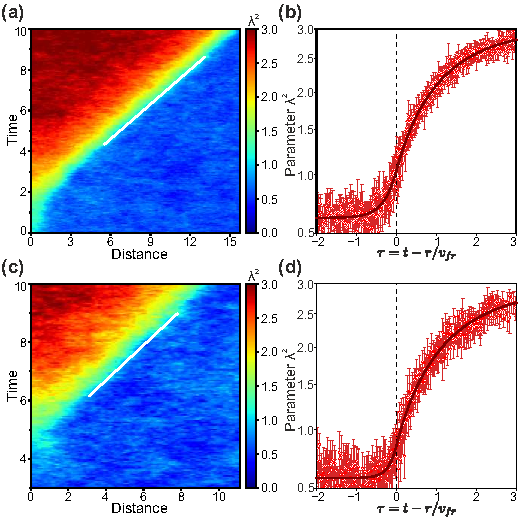
\includegraphics[width=100mm]{SSMF-Figure6.pdf}
 \caption{\textbf{Автомодельные фронты при росте сверхкритического и спонтанно образовавшегося зародыша}:
 Эволюция поля $ \lambda^2$ в радиальных направлениях, показанных белыми стрелками на Рис.~\ref{SSMF-Figure5} (b2) и \ref{SSMF-Figure5} (c2) для (a, b) сверхкритических и (c, d) спонтанно образованных начальных флуктуаций.
  Графики (a, c) и (b, d) получены таким же образом, как (d, e) на Рис.~\ref{SSMF-Figure2} и \ref{SSMF-Figure3}.}
\label{SSMF-Figure6}
\end{figure}

%\subsubsection{Бифуркационное поведение $\lambda^2$ -поля и нуклеационное поведение}
%\label{SSMF-Results-Modeling}

Как известно, процесс зародышеобразования при плавлении состоит из трех стадий \cite{10.1038/ncomms7942}: (i) пребывание перегретого кристалла в метастабильном состоянии до образования критических зародышей (например, дефектов \cite{10.1038/nmat1375} или петель диффундирующих частиц \cite{10.1103/physrevb.77.134109}), (ii) образование критических зародышей \cite{10.1126/science.1224763, 10.1063/1.2790424, 10.1063/1.2424715},  (iii) рост посткритических зародышей (изображено на Рис.~\ref{SSMF-Figure2} и \ref{SSMF-Figure3}).
Флуктуации $\lambda^2$, обусловленные наличием в уравнении~\eqref{SSMF-eq6} источника теплового шума $\xi(t, \mathbf{r})$, влияют на распространение фронта плавления. Это вызвано высокой восприимчивостью системы к флуктуациям вблизи фазового перехода.
Переход происходит при $\lambda_{\mathrm{cr}}^2=\lambda_\ast^2$,
и некоторые флуктуации вблизи фронтов плавления влияют на распространение фронта, как показано на Рис.~\ref{SSMF-Figure2} (d) и \ref{SSMF-Figure3} (d).
Однако флуктуации $\lambda^2$ на начальных этапах зарождения могут повлиять на эволюцию системы еще сильнее.

Чтобы проиллюстрировать нетривиальное бифуркационное поведение модели \eqref{SSMF-eq6}, чувствительной к эффектам теплового шума и структуре исходного $\lambda^2$-распределения, было рассмотрено и численно решено стохастическое дифференциальное уравнение в частных производных, следующее из уравнения~\eqref{SSMF-eq6} и \eqref{SSMF-eq7}:
\begin{equation}
\label{SSMF-eq10}
\begin{split}
& \partial_t \lambda^2 = \nabla^2\lambda^2 + Q (\lambda^2) +  \varepsilon^{1/2}\xi(t,\mathbf{r}), \\
& Q(\lambda^2) = -(\lambda^2-\lambda_1^2) + (\lambda_2^2-\lambda_1^2)\eta(\lambda^2-1),
\end{split}
\end{equation}
где $\lambda^2$ нормировано на $\lambda_\ast^2$, $\lambda^2/\lambda^2_\ast \rightarrow \lambda^2$,
время $t\gamma \rightarrow t$, и расстояние  $r \sqrt{\gamma/\chi} \rightarrow r$,
и для простоты предполагается, что $\chi_{1,2}=\chi$, $\gamma_{1,2} = \gamma$;
$\eta(s)=(1+\exp(-100 s ))^{-1}$ это сглаженная ступенчатая функция Хевисайда,
и $\left<\xi(t,\mathbf{r})\xi(t',\mathbf{r}')\right>=\delta(t-t')\delta(\mathbf{r}-\mathbf{r'})$.
Таким образом, в уравнении~\eqref{SSMF-eq10} свободными параметрами остаются величина теплового шума $ \varepsilon $ и нормированные параметры $\lambda^2_{1,2}$
Расчет был выполнен при значениях $\lambda_1^2 = 0.6$ и $\lambda_2^2 = 3.0$, полученных из эксперимента.

Уравнение~\eqref{SSMF-eq10} было решено с использованием гауссовых начальных распределений $ \lambda ^ 2$:
\begin{equation}
\label{SSMF-eq11}
\lambda^2(0, \mathbf{r}) = \lambda^2_1 + \delta\lambda^2 \exp\left(-\frac{\mathbf{r}^2}{l^2}\right),
\end{equation}
где величина $ \delta\lambda^2$ изменялась в диапазоне от $ 0 $ до $ 1.5 $, a $ l ^ 2 = 0.4 $ в 1D и $ l ^ 2 = 1 $ в 2D случае.
Размеры системы были выбраны равными $20$ и $20 \times 20 $ в 1D и 2D случае соответственно, и на ее границах поддерживались фиксированные значения $\lambda^2= \lambda_1 ^ 2 $.
Уравнение \eqref{SSMF-eq10} решалось с помощью экспоненциальной схемы Эйлера~\cite{10.1098/rspa.2008.0325}, используя временной шаг $\Delta t=10^{-3}$ ($\Delta t=5\times10^{-4}$) и
2048 ($512\times512$) собственные функции в 1D (2D) случае. \textcolor{red}{В трехмерном случае мы рассматривали систему с размерами $31.62 \times 31.62 \times 31.62$, используя временной шаг $\Delta t = 5 \times 10 ^ {-4}$ и собственные функции $128 \times 128 \times 128 $.}

\textcolor{red}{Следует отметить, что говоря о размерах задачи, мы имеем в виду симметрию ядер. Таким образом, уравнения записываются в одинаковой форме для двухмерных или трехмерных систем плавления, а различие связано с формой операторов $\nabla ^ 2$ в двухмерном и трехмерном случаях в уравнении ~\eqref{SSMF-eq10}. Таким образом, настоящие результаты соответствуют 3D перегретым кристаллам. Представленные результаты для одномерного и двухмерного случаев следует рассматривать как трехмерную систему с плоским фронтом плавления, движущимся в одном направлении, и цилиндрически расширяющимся, соответственно.}

Для иллюстрации бифуркационного поведения, приводящего к зарождению и формированию устойчивых фронтов плавления, рассмотрена эволюция поля $\lambda^2$ с начальным распределением \eqref{SSMF-eq11} при различных значениях $ \delta\lambda^2$.
\textcolor{red}{Результаты при $ \varepsilon = 0 $ для случаев 1D, 2D и 3D систем представлены на Рис.~\ref{SSMF-Figure4}.}
Временные зависимости $\lambda^2(t, 0) $ показаны на Рис.~\ref{SSMF-Figure4}.
В зависимости от величины $\delta\lambda^2$ (или $\lambda_0^2 \equiv \lambda^2(0,0)=\lambda_1^2 + \delta \lambda^2$), решение демонстрирует бифуркационное поведение с критическими значениями $\lambda^2_{0,\mathrm{cr}} \simeq 1.09$ в 1D случае, $\lambda^2_{0,\mathrm{cr}}\simeq 1.29$ в 2D \textcolor{red}{и $\lambda^2_{\mathrm{cr}}\simeq 2.2$ в 3D системе.}
Флуктуации с $ \lambda_0 ^ 2 <\lambda ^ 2_ {0, \mathrm{cr}} $ исчезают, система стремится к (кристаллическому) состоянию с малым $\lambda^2$, а флуктуации с $\lambda_0^2> \lambda^2_{0, \mathrm{cr}}$ переходят в состояние с большим $\lambda^2$ (жидкость).
При $\lambda_0^2>\lambda^2_{0, \mathrm{cr}}$ бифуркационное поведение также зависит от начального значения $\lambda_0^2$, и это наиболее очевидно для верхних кривых на Рис.~\ref{SSMF-Figure4}(a) и \ref{SSMF-Figure4}(b), для которых характерно уменьшение значения $ \lambda_0^2 $ на начальном этапе эволюции, за которым следует резкий рост с переходом в жидкое состояние.
\textcolor{red}{Ниспадающее начальное падение отражает передачу энергии соседям от центральных частиц в исходном узле $\lambda^2 (0,0)$. Мы видим, что наибольшая начальная $\lambda ^ 2$ -- флуктуация, способная вызвать фазовый переход, соответствует трехмерным ядрам. Это ожидается, поскольку образование зародышей регулируется взаимодействием между процессами формирования поверхности (связанными с членом $(\nabla \lambda ^ 2) ^ 2$ в уравнении ~\eqref{SSMF-eq5}) и высвобождением свободной энергии (описывается источником $Q (\lambda ^ 2)$ в процессе эволюции системы).}

Слабый тепловой шум незначительно влияет на эволюцию околокритических начальных состояний.
Критические значения $\lambda^2_{0,\mathrm{cr}}$ зависят от конкретного выбора профиля начальной флуктуаций (что связано с градиентами $\lambda^2$) и (немного) от размерности системы.
Однако бифуркации делают задачу существенно нелинейной:
результирующий сценарий эволюции $\lambda^2$ определяется балансом между эффектами генерации и диссипации $\lambda^2$ в уравнении~\eqref{SSMF-eq10}.
В общем случае, из-за кривизны пространственно-неоднородных $\lambda^2$-флуктуаций (цилиндрический или сферический зародыш), $\lambda_{\mathrm{cr}}^2 > \lambda_\ast^2$.





Эффекты теплового шума проиллюстрированы на Рис.~\ref{SSMF-Figure5} на основе результатов, полученных при различных начальных флуктуациях, а также для случая спонтанного (индуцированного тепловыми флуктуациями) зародышеобразования в гомогенной системе.
Рис.~\ref{SSMF-Figure5}(a) и \ref{SSMF-Figure5}(b) демонстрируют снимки временной эволюции флуктуаций с $\lambda^2_0 \lessgtr \lambda^2_{0,\mathrm{cr}}$.
Эти результаты соответствуют случаям $\lambda_0^2 =1.28$ и $1.3$ на Рис.~\ref{SSMF-Figure4}(c) при $\varepsilon = 10^{-4}$.
Начальные условия расчета показаны на Рис.~\ref{SSMF-Figure5}(a1), \ref{SSMF-Figure5}(b1),
тогда как эволюция систем проиллюстрирована на Рис.~\ref{SSMF-Figure5}(a2-a5) и \ref{SSMF-Figure5}(b2-b5).
Видно, что тепловой шум может влиять на форму околокритического зародыша и форму фронта плавления, как показано на Рис.~\ref{SSMF-Figure5}(b4).
Однако на следующих этапах эволюции, зародыши становятся симметричными, как показано на Рис.~\ref{SSMF-Figure5}(b5).
Такое же поведение наблюдалось в экспериментах по росту жидких зародышей при гомогенном плавлении коллоидных кристаллов \cite{10.1038/ncomms7942}.

Процесс самопроизвольного зародышеобразования в изначально однородном случае показан на Рис.~\ref{SSMF-Figure5}(c).
Эти результаты иллюстрируют численное решение уравнения~\eqref{SSMF-eq10} при однородном начальном распределении $\lambda_0^2 = 0.6$ и при $\varepsilon=5.8\times10^{-4}$.
При достаточно сильном тепловом шуме флуктуационный механизм обеспечивает спонтанное образование критического зародыша, показанного на Рис.~\ref{SSMF-Figure5}(c3).
Рост зародышей сопровождается образованием жидких зародышей перед фронтом плавления, таким же образом, как это наблюдается в экспериментах и моделировании методом МД.


Результаты моделирования эволюции $\lambda^2$, показанные на Рис.~\ref{SSMF-Figure5}(b) и \ref{SSMF-Figure5}(c), были обработаны в выбранных направлениях (обозначены на Рис.~\ref{SSMF-Figure5} белыми стрелками), таким же образом, как это было сделано с экспериментальными и МД данными, показанными на Рис.~\ref{SSMF-Figure2} и \ref{SSMF-Figure3}.
Результаты обработки, представленные на Рис.~\ref{SSMF-Figure6}(a) и \ref{SSMF-Figure6}(b), соответствуют росту критического зародыша, показанному на Рис.~\ref{SSMF-Figure5}(b). На Рис.~\ref{SSMF-Figure6}(a) отчетливо видно формирование фронта плавления из исходного зародыша.
Аналогичное поведение наблюдалось экспериментально в комплексной (пылевой) плазме, как описано в работе~\cite{10.1103/physreve.97.043206}, что подтверждает найденную здесь аналогию.

После того как фронт плавления сформирован, $\lambda^2$ -профиль описывается двумя экспоненциальными ветвями, как это и ожидалось (сплошная красная линия на рис.~\ref{SSMF-Figure6}(b)).
Результаты для гомогенного зародышеобразования (рис.~\ref{SSMF-Figure5}(c)) показаны на Рис.~\ref{SSMF-Figure6} (c) и \ref{SSMF-Figure6}(d).
В этом случае поле $\lambda^2$ сильно флуктуирует из-за повышенного теплового шума, и фронт плавления немного более размыт в пространстве (зеленая полосой на рис.~\ref{SSMF-Figure6}(c)), но общее поведение аналогично Рис.~\ref{SSMF-Figure6}(a) и \ref{SSMF-Figure6}(b).
Таким образом, самосогласованность предложенной $\lambda^2$-модели становится наглядно продемонстрированной: экспериментальные результаты, представленные на Рис.~\ref{SSMF-Figure2} и \ref{SSMF-Figure3} и описанные уравнением~\eqref{SSMF-eq6}, воспроизводятся на рисунках~\ref{SSMF-Figure5} и \ref{SSMF-Figure6}, полученных на основе уравнения~\eqref {SSMF-eq10}.

\begin{figure*}[!t]
\centering
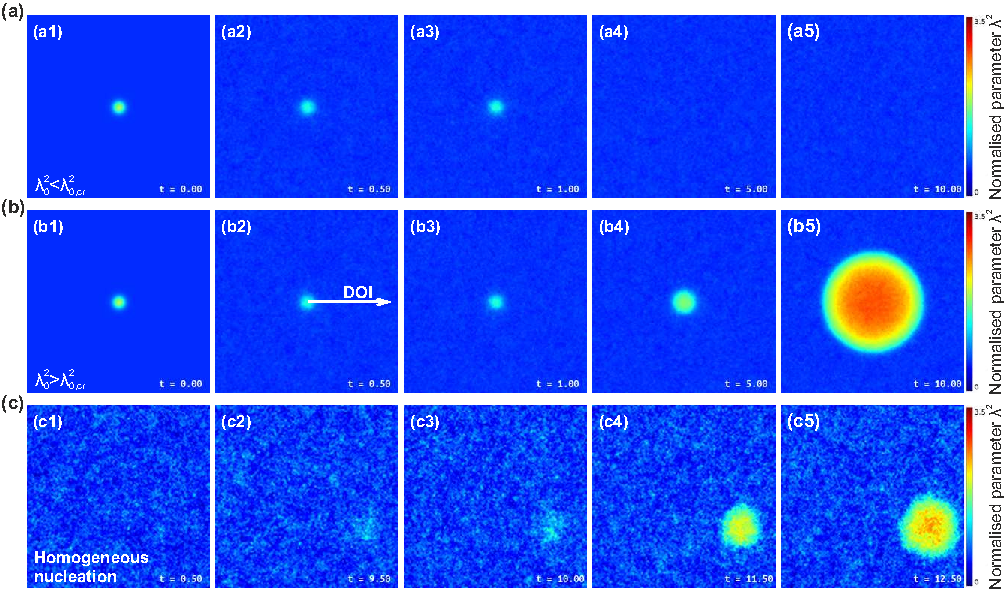
\includegraphics[width=170mm]{SSMF-Figure7.pdf}
 \caption{\textcolor{red}{\textbf{Эволюция различных начальных трехмерных (сферических) $\lambda^2$~-~флуктуаций (ядер) и спонтанное зарождение в однородной системе}:
Последовательные кадры иллюстрируют эволюцию (a) докритической и (b) сверхкритической $\lambda^2$ -флуктуации (ядра) и спонтанное зарождение ядра из-за теплового шума.}}
\label{SSMF-Figure7}
\end{figure*}

\begin{figure}[!t]
\centering
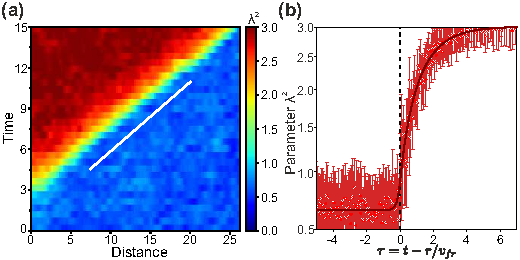
\includegraphics[width=85mm]{SSMF-Figure8.pdf}
 \caption{\textcolor{red}{\textbf{Автомодельный фронт при росте ядра в трехмерной системе}:
Эволюция $\lambda^2$~-~поля в радиальных направлениях, показанных белыми стрелками на Рис.~\ref{SSMF-Figure7}(b2) для сверхкритического ядра.
(a) и (b) получены таким же образом, как (d, e) на Рис.~\ref{SSMF-Figure2} и \ref{SSMF-Figure3}.}}
\label{SSMF-Figure8}
\end{figure}

\textcolor{red}{Тенденции, которые мы наблюдали для эволюции двумерных ядер, качественно такие же, как и в трехмерном случае, когда мы рассматриваем сферические ядра, как показано на Рис.~\ref{SSMF-Figure7} и \ref{SSMF-Figure8}. Здесь поперечные сечения системы показаны на Рис.~\ref{SSMF-Figure7}(a) и \ref{SSMF-Figure7}(b), чтобы проиллюстрировать зарождение суб- и сверхкритических ядер при $\lambda_0^2 = 2.21$ и $\lambda_0^2 = 2.23$ соответственно.
Общая картина эволюции кластера полностью такая же, как и в случае 2D. Случай гомогенного зародышеобразования показан на рис.~\ref{SSMF-Figure7}(c), где видно, что сильные тепловые флуктуации могут образовывать активированный кластер, способный к индуцированию фазового перехода через распространяющиеся фронты плавления. Последний проиллюстрирован на Рис.~\ref{SSMF-Figure8} так же, как на Рис.~\ref{SSMF-Figure6}(a) и \ref{SSMF-Figure6}(b).
На Рис.~\ref{SSMF-Figure8}(a) видно, что после образования зародыша оно растет линейно. $\lambda ^ 2$ --профиль на больших расстояниях от центра зародышеобразования рассчитывался так же, как на Рис.~\ref{SSMF-Figure2}, \ref{SSMF-Figure3} и \ref{SSMF-Figure6}, и результат показан на Рис.~\ref{SSMF-Figure8}(b): опять же, $\lambda ^ 2$ -- профиль состоит из двухэкспонентных ветвей (показаны сплошной красной линией) в полное согласие с нашими экспериментами и результатами МД, обсуждавшимися ранее. Таким образом, предложенная модель среднего поля последовательно описывает зарождение и бифуркационное поведение $\lambda ^ 2$ - поля в 1D, 2D и 3D системах.}

%\subsection{\textcolor{red}{Выводы}}

В итоге, в рамках первого этапа настоящего проекта предложена модель среднего поля, для описания  плавления, основанная на новом параметре порядка $\lambda^2$ -- среднеквадратичном отклонении расстояний между частицами в соседних ячейках Вороного.
Поведение поля $\lambda^2$ было проанализировано с использованием нестационарного уравнения Гинзбурга-Ландау с тепловым шумом и источниками.
Показано, что разработанная модель демонстрирует существенно нелинейное поведение, в то время как слагаемые в уравнениях имеют ясный физический смысл в контексте анализа плавления кристаллов.
Это было продемонстрировано путем анализа экспериментальных данных с использованием систем с разными режимами динамики движения частиц -- броуновским в коллоидах и ньютоновским в MD моделировании, а так же на основе последующего сравнения с моделью, демонстрирующей превосходное описание распространения фронтов плавления и их структуры.
Кроме того, будучи по своей сути микроскопической, предложенная модель позволяет с высокой степенью детализации изучать зародышеобразование в различных режимах перегрева (в зависимости от величины теплового шума) и эволюцию реалистичных жидких зародышей, которые могут принимать самые разные сложные формы.

При помощи экспериментов с плавлением коллоидных кристаллов NIPAm частиц и МД-моделирования перегретых кристаллов типа твердой сферы, образованных частицами c IPL18 взаимодействием, доказано, что профиль $\lambda^2 $ стационарных фронтов состоит из двух экспоненциальных ветвей.
Предложенная модель демонстрирует бифуркационное поведение, присущие начальным стадиям процесса зародышеобразования, и позволяет полностью восстановить процесс зародышеобразования в гомогенной системе и кинетику фронта плавления.
Удалось обнаружить, что предложенная модель обеспечивает четкую аналогию между фронтами плавления в перегретых коллоидных и атомарных кристаллах и неравновесным плавлением в комплексной (пылевой) плазме, а также с фронтами реакции в экзотермических химически реактивных средах.
Таким образом, предложенная теоретическая модель может послужить основой для изучения широкого круга явлений в различных системах, от атомных и молекулярных до коллоидных и белковых систем.

Процесс зародышеобразования в перегретых кристаллах, кинетика образования и роста жидких зародышей и структура устойчивых фронтов плавления представляют собой центральные проблемы для понимания плавления кристаллов.
Представленные результаты являются существенным шагом вперед, предоставляя простой и эффективный инструмент для изучения процессов зародышеобразования и плавления в перегретых кристаллах различной природы.
%Это должно быть интересно широкому кругу специалистов в области конденсированных сред, материаловедения, химической физики и мягкой материи.


%Предложенная модель до сих пор тестировалась в случае 2D, однако качественно аналогичное поведение ожидается и для 3D-систем.
%В этом случае понятие $\lambda^2$ -поля следует обобщить на объемные структуры, и это можно сделать, заменив ячейки Вороного соответствующими многогранниками.
%Поскольку $\lambda^2$ напрямую связано со вторым кумулянтом первого пика в парной корреляционной функции,
%что представляет собой важное преимущество для будущих экспериментов с типичными атомными системами, где $\lambda^2$ может быть получено, например, из данных рассеяния рентгеновских лучей или нейтронов.
%Поле вторых кумулянтов можно также извлечь экспериментально, например, с помощью
%расширенной тонкой структуры поглощения рентгеновских лучей (EXAFS) \cite{10.1016/0167-5087(83)90655-5, 10.1107/s0909049501014923, 10.1103/physrevb.56.11531, 10.1103/physrevb.65.172104, 10.1103/physrevb.70.174301, 10.1088/0953-8984/13/7/201}.
%Это дает прекрасную возможность экспериментально измерить $\lambda^2$ -поведение на реальных материалах, обеспечивая путь для экспериментального изучения плавления, в том числе в экстремальных условиях.

%В более широком смысле предлагаемая модель открывает широкие перспективы для изучения
%плавления, а также кристаллизации,
%статистического анализа процесса нуклеации,
%зарождение при разных режимах перегрева, от слабого до сильного, и, в частности,
%флуктуационные механизмы, ответственные за ускорение фронтов плавления в сильно перегретом режиме \cite{10.1038/ncomms7942}.
%Предлагаемый подход может быть обобщен на различные случаи, включая системы анизотропных и активных частиц.
%Кроме того, благодаря своей формулировке предлагаемая модель одинаково подходит для анализа плавления в стеклообразных системах, а также для анализа механизма стеклования - одной из давних проблем в науке о конденсированных средах и мягких веществах.
%Соответствующие теоретические и экспериментальные исследования важны для
%понимания роли диффузии и теплового шума в переходе от медленно распространяющихся фронтов плавления к быстро распространяющимся, и процесса зародышеобразования.
%Однако мы оставляем эти интересные задачи для будущих работ.

